\chapter{Platforma od strony technicznej}
\label{chapter:platform-technical}
Ogólny schemat platformy wraz z użytymi technologiami został przedstawiony na rysunku \ref{fig:platform-schema}.

\begin{figure}[h]
    \centering
    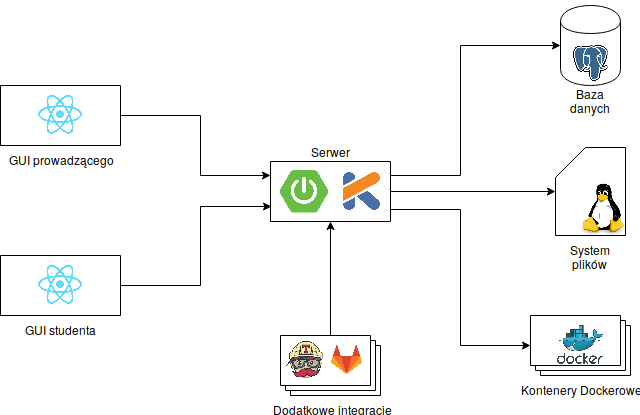
\includegraphics[width = 13cm]{chapter02/platform_schema.png}
    \caption{Schemat platformy i użytych technologii (źródło własne).}
    \label{fig:platform-schema}
\end{figure}

Platforma składa się z dwóch webowych interfejsów graficznych: interfejsu prowadzącego oraz studenta.
Oba interfejsy zostały napisane w technologii ReactJS z użyciem MaterialUI.

Moduł serwera został napisany w języku Kotlin z użyciem SpringBoot’a w wersji 2.0.

Serwer przechowuje dane w formie rekordów w bazie danych oraz plików.
Metadane, takie jak termin prowadzącegorealizacji wskazanego etapu lub grupy, do których są przypisani studenci, są przechowywane w bazie PostgreSQL.
Dane w postaci plików są przechowywane na dysku w systemie plików Linux.

Programy studentów są uruchamiane w kontenerach Dockerowych.

Platformę można zintegrować z zewnętrznymi narzędziami.
Przykładem takiej integracji może być repozytorium kodu oraz system CI (ang. Continious Integration).
System CI (przykładowo Travis) można skonfigurować w taki sposób, aby bezpośrednio po zaakceptowaniu PR (ang. Pull Request) do repozytorium kodu (przykładowo GitLab) uruchamiany był job, który po poprawnym zbudowaniu programu automatycznie przesyłał go do platformy i uruchamiał.

\section{Schemat bazy}

Schemat bazy danych znajduje się na rysunku \ref{fig:platform-db-schema}.

\begin{figure}[h]
    \centering
    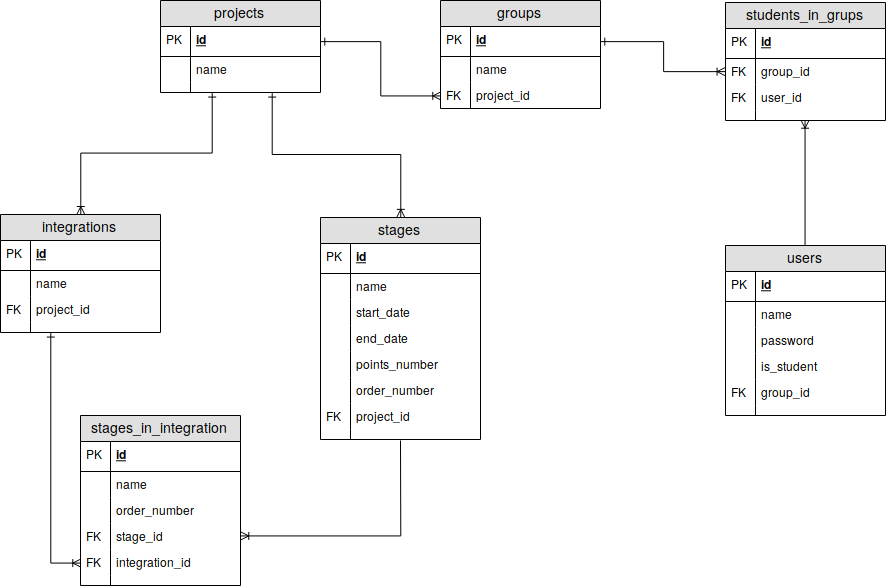
\includegraphics[width = 13cm]{chapter02/db_schema.png}
    \caption{Schemat bazy danych (źródło własne).}
    \label{fig:platform-db-schema}
\end{figure}

TODO: Opisać schemat i napisać o archiwizacji danych

\section{Schemat katalogów plików}

Schemat katalogów plików znajduje się na rysunku \ref{fig:platform-directories}.

\begin{figure}[h]
    \centering
    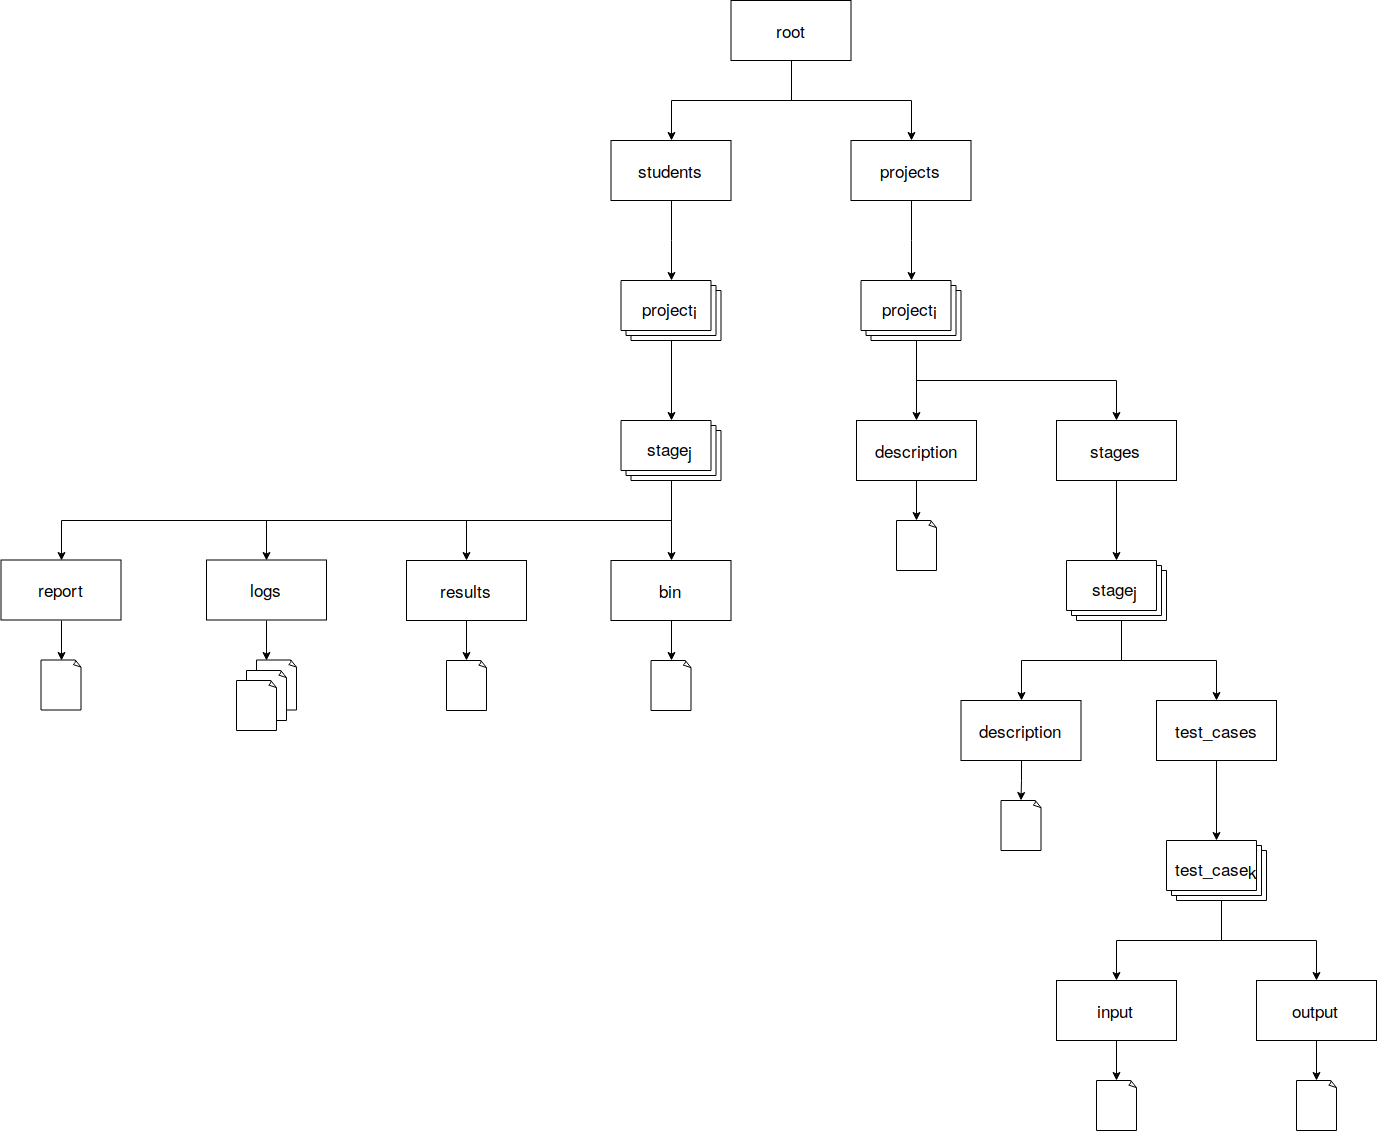
\includegraphics[width = 13cm]{chapter02/directories.png}
    \caption{Schemat katalogów plików (źródło własne).}
    \label{fig:platform-directories}
\end{figure}

TODO: Opisać schemat i napisać o archiwizacji danych

\section{Uruchomianie i testowanie programów studentów}

Programy studentów są uruchamiane w kontenerach Dockerowych.
Obraz środowiska jest ustalany dla zadanego projektu.
Technologia Docker jest szeroko używana komercyjnie.
Dzięki temu charakteryzuje się ona wysoką niezawodnością i stabilnością.
Również biblioteki OpenSource ułatwiające uruchamianie kontenerów Dockerowych bezpośrednio z kodu Javowego są szeroko stosowana i dobrze przetestowane.
Samo uruchamianie kontenerów, ich integracja oraz konfiguracja nowych środowiska, jest szybka i stosunkowo prosta.

\begin{figure}[h]
    \centering
    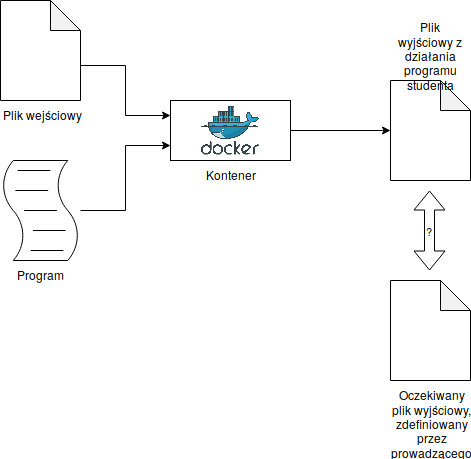
\includegraphics[width = 13cm]{chapter02/single_test_case.png}
    \caption{Schemat sprawdzenia poprawności działania programu studenta (źródło własne).}
    \label{fig:single-test-case}
\end{figure}

Schemat sprawdzenia poprawności działania programów studentów został przedstawiony na rysunku \ref(fig:single-test-case).
Po uruchomieniu programu studenta na platformie, uruchamiane są wszystkie przypadki testowe dla zadanego etapu.
Uruchomienie pojedynczego przypadku testowego sprowadza się do utworzenia nowego kontenera Dockerowego i podania mu jako volumenu ścieżki do programu studenta oraz ścieżki do pliku wejściowego.
Program studenta jest uruchamiany dla zadanych danych wejściowych w kontenerze.
Oczekuje się, że program studenta w wyniku swojego działania utworzy plik wyjściowy.
Zawartość tego pliku zostanie porównana z zawartością oczekiwanego pliku wejściowego dla danego przypadku testowego. Jeśli dane są zgodne, przypadek testowy uważa się za spełniony.

\begin{figure}[h]
    \centering
    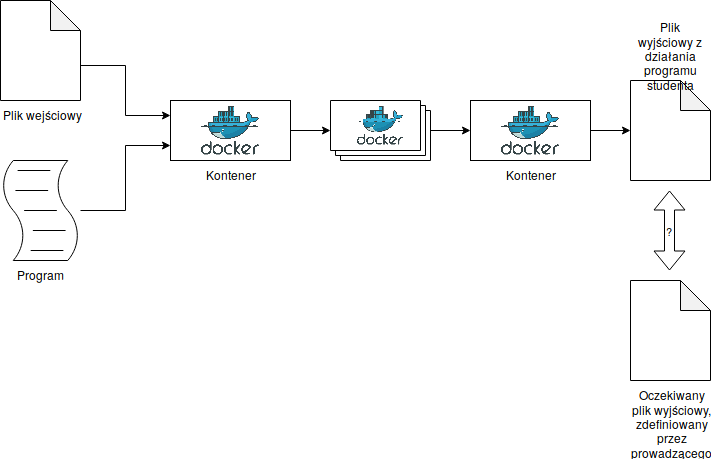
\includegraphics[width = 13cm]{chapter02/integration.png}
    \caption{Schemat sprawdzenia poprawności procesu integracji programów studentów (źródło własne).}
    \label{fig:integration}
\end{figure}

Schemat przebiegu procesu integracji został przedstawiony na rysunku \ref(fig:integration).
Prowadzący definiuje kolejne etapy wykonywane w ramach procesu integracji.
Przebieg procesu integracji jest bardzo podobny do wykonania pojedynczego przypadku testowego.
Różnica polega na tym, że plik wyjściowy utworzony w wyniku uruchomienia poprzedniego etapu jest plikiem wejściowym dla kolejnego, następującego po nim.
Plik wyjściowy dla ostatniego etapu jest porównywany ze zdefiniowanym oczekiwanym plikiem wyjściowym.

\section {Konfiguracja uruchomieniowego środowiska Dockerowego}

TODO: Opis i przykład

\section {Uwierzytelnienie użytkowników}

TODO: opis:
1) proste uwierzytelnienie oparte o login i hasło
2)prosta autoryzacja oparta o nadanie praw administratora prowadzącym
oraz ograniczenie praw wykonania studentom,

\section {Zestawienie platformy na serwerze}

TODO: Opis i przykład

\section {Przykład integracji platformy z narzędziem CI oraz repozytorium kodu}

TODO: opis i przykład integracji platformy z narzędziem CI oraz repozytorium
kodu.